% =============================================================================
% Mostly Noise: Privacy-Budget Allocation and Trust-Based Robustness in
% Differentially Private Federated Drone Detection
% Source of every number: restart/ (see restart/paper/TRACEABILITY.md).
% Template: IEEEtran, journal mode (long form), per author choice 2026-10-12.
% =============================================================================
\documentclass[journal]{IEEEtran}
\usepackage[utf8]{inputenc}
\usepackage[T1]{fontenc}
\usepackage{amsmath,amssymb,amsthm}
\usepackage{graphicx}
\usepackage{booktabs}
\usepackage{multirow}
\usepackage{array}
\usepackage{xcolor}
\usepackage{url}
\usepackage{cite}
\newtheorem{proposition}{Proposition}
\newtheorem{assumption}{Assumption}
\newcommand{\missing}[1]{\textcolor{red}{[MISSING: #1]}}
\newcommand{\verify}[1]{\textcolor{orange}{[VERIFY: #1]}}
\newcommand{\eps}{\varepsilon}
\newcommand{\mAP}{mAP@0.5}

\begin{document}

\title{Mostly Noise: Privacy-Budget Allocation and Trust-Based Robustness in Differentially Private Federated Drone Detection}

\author{\missing{author names and affiliations}}

\markboth{Manuscript draft, 2026-10-12}{Mostly Noise: DP Federated Drone Detection}

\maketitle

% -----------------------------------------------------------------------------
\begin{abstract}
How to spend a privacy budget over training rounds, and how to aggregate updates when some clients
are malicious, are usually studied separately and at weak privacy. We study both on one
differentially private (DP) federated infrared drone detector at worst-client $\eps = 0.79$--$2.72$
($\delta=10^{-5}$, frame-level), with pre-registered rules, 20 paired seeds and Holm correction. At
$\eps = 1.86$ an honest update's cosine with a clean server update is 0.0075. A fixed schedule with
less noise in later rounds beats uniform allocation by $+0.0139$ \mAP{} [$+0.0076$, $+0.0202$]
($+23.5\%$, 16/20 seeds). Reinforcement learning, Bayesian optimisation and a constrained learned
policy add nothing. FLTrust loses 75\% of accuracy without attack. A noise-aware rescaling restores
it, but a rule-aware attacker drives it to 0.0005 \mAP{}, and capping each client's trust weight at
1/8 still leaves 0.0058. Limitation: one primary dataset, frame-level privacy, low absolute accuracy
(uniform 0.059 \mAP). Central claim: \emph{at strong privacy an honest DP update is almost entirely noise; consequently, all the
allocation gain we could measure comes from placing less noise in later rounds, which a fixed
schedule already captures, while trust-based robust aggregation either drowns the honest signal or
hands control to a coherent attacker.}
\end{abstract}

\begin{IEEEkeywords}
Differential privacy, federated learning, privacy-budget allocation, Byzantine robustness, FLTrust,
adaptive attacks, object detection, pre-registration.
\end{IEEEkeywords}

% -----------------------------------------------------------------------------
\section{Introduction}
\label{sec:intro}

Consider eight operators of counter-drone infrared cameras: airports, border posts, and sites near
buildings, hills and cloud-heavy sky. Each holds footage that cannot leave its premises, and each
wants a better drone detector than its own data can train. Federated learning (FL)~\cite{mcmahan2017fedavg}
keeps the footage local. DP-SGD~\cite{abadi2016dpsgd} bounds what the shared model reveals about
any single frame. Two questions then decide whether the system is worth deploying. First, the
privacy budget is fixed, so how should it be spent over training rounds? Second, some operators may
be compromised, so which aggregation rule protects the model?

Both questions have active literatures, but they are studied apart and mostly at weak privacy.
Time-adaptive budget allocation~\cite{kiani2025timeadaptive} reports gains at $\eps = 10$--$30$
from three-run averages without significance tests. Byzantine-robust aggregation rules such as
Krum~\cite{blanchard2017krum}, the coordinate-wise median~\cite{yin2018median} and
FLTrust~\cite{cao2021fltrust} are designed and evaluated mostly without DP noise. Guerraoui et
al.~\cite{guerraoui2021dpbyz} show theoretically that the two kinds of guarantee interact badly as
the model dimension grows. What practitioners lack is a controlled, statistically careful
measurement of both choices on one realistic task at the privacy levels a regulator would accept.

This paper provides that measurement. Its central claim is: \emph{at strong privacy an honest DP
update is almost entirely noise; consequently, all the allocation gain we could measure comes from
placing less noise in later rounds, which a fixed schedule already captures, while trust-based
robust aggregation either drowns the honest signal or hands control to a coherent attacker.}

\textbf{Contributions.} Each is stated with its measured result; all comparisons use 20 paired
seeds and pre-registered decision rules.
\begin{enumerate}
  \item \emph{Measured noise dominance.} At $\eps = 1.86$ an honest client update has norm 41.4,
  against 1.06 for the server's clean update, and cosine 0.0075 with it. The cosine falls
  monotonically from 0.086 without DP to 0.0033 at $\eps = 0.79$ (Fig.~\ref{fig:mechanism}).
  \item \emph{Allocation: placement matters, learning does not.} Round sensitivity rises in late
  rounds in 7 of 9 tested configurations and is flat in none. A one-parameter decaying schedule beats
  uniform by $+0.0139$ \mAP{} ($+23.5\%$, 16/20 seeds) at $\eps = 1.86$. A DDPG agent collapses
  (0.000), and a TD3+GRU agent ties uniform ($-0.0005$). Bayesian optimisation (BO) and a TD3 agent
  constrained to $\pm20\%$ around the theory schedule tie the fixed schedules. Neither of two
  server-side feedback signals carries usable information (Section~\ref{sec:res-learn}).
  \item \emph{More rounds do not help at fixed $\eps$.} At $\eps = 1.86$ the tuned schedule scores
  0.073 / 0.086 / 0.057 / 0.040 at 12 / 25 / 50 / 100 rounds. Over the same range the no-DP model
  rises to 0.33--0.34, so the private model's share of it falls from 29\% to 12\%.
  \item \emph{Trust-based robustness fails under DP and is only partly repairable.} FLTrust loses to
  FedAvg at every $\eps$ from 30.16 to 0.79, including without attack ($-75\%$ at $\eps = 1.86$). A
  noise-aware norm target (Variant N) recovers FedAvg-level accuracy at $\eps = 1.86$. An attacker who
  knows the rule drives it to 0.0005 \mAP{}, a loss against FedAvg ($-0.013$, 1/18 wins). Capping any
  client's trust weight at 1/8 holds the attackers at exactly 25\% of the weight, but the model still
  collapses (0.0058).
  \item \emph{An auditable negative-results record.} The record holds every pre-registered prediction
  that failed, one retraction (an FL$\times$DP interaction whose sign reversed once the clipping
  bound was calibrated), and every discarded implementation (Section~\ref{sec:res-failed}).
\end{enumerate}

\textbf{Scope and limitations.} All security results and the main allocation results use one
dataset (Anti-UAV infrared~\cite{zhao2023antiuav}). Allocation is replicated on VisDrone~\cite{zhu2022visdrone} and
CIFAR-10~\cite{krizhevsky2009cifar}. Privacy is frame-level, and consecutive frames of one recording are correlated, so the
guarantee for a whole recording is weaker than the stated $\eps$. The trainable model is small
(65,221 parameters on a frozen backbone), and absolute accuracy on the held-out test sessions is low
(0.059 \mAP{} for uniform at $\eps = 1.86$). The adaptive attacker is omniscient. These limits are
detailed in Section~\ref{sec:limits}.

% -----------------------------------------------------------------------------
\section{Related Work}
\label{sec:related}

\textbf{DP training and accounting.} DP-SGD~\cite{abadi2016dpsgd} clips per-sample gradients and adds
Gaussian noise. R\'enyi DP~\cite{mironov2017rdp} and concentrated DP~\cite{bun2016zcdp} give tight
composition, and Opacus~\cite{yousefpour2021opacus} implements Poisson-subsampled RDP accounting,
which we use throughout. User-level DP for FL was introduced by McMahan et al.~\cite{mcmahan2018dplm};
our unit is the frame, which is weaker (Section~\ref{sec:limits}). Hyper-parameter tuning itself
leaks privacy~\cite{papernot2022hyperparam}; we do not account for it (Section~\ref{sec:limits}).

\textbf{Time-adaptive privacy spending.} Kiani et al.~\cite{kiani2025timeadaptive} propose
``spend-as-you-go'': clients save budget early by sampling less, then spend it later. They report
gains over uniform DP-FedAvg at client-level $\eps = 10$--$30$ on MNIST, FMNIST and Adult, averaged
over three runs. Our results \emph{agree} with their direction (less noise late is better) and do
not contradict their numbers, which come from a different regime. We add three things: a direct
measurement of why late rounds matter (a noise-pulse test); paired, corrected statistics; and tests
of learned and searched schedules, which they do not evaluate. Their rule, implemented in our
setting, is the worst arm on CIFAR-10 but wins on VisDrone (Section~\ref{sec:res-alloc}).

\textbf{Learned allocation.} Reinforcement-learning agents that set per-round noise use actor-critic
methods such as DDPG~\cite{lillicrap2016ddpg} and TD3~\cite{fujimoto2018td3}. We test both, with the
agents trained only on public data so that training spends no client privacy.

\textbf{Byzantine-robust FL and attacks.} Krum~\cite{blanchard2017krum} and the coordinate-wise
median~\cite{yin2018median} bound the influence of outliers. FLTrust~\cite{cao2021fltrust}
bootstraps trust from a small clean root dataset at the server: each update is weighted by the
ReLU of its cosine with the server's root update and rescaled to the root update's norm. We use
three standard attacks: ALIE~\cite{baruch2019alie}, inner-product manipulation
(IPM)~\cite{xie2019ipm}, and Fang et al.'s full-knowledge attack~\cite{fang2020localpoison}.

\textbf{DP and robustness together.} Guerraoui et al.~\cite{guerraoui2021dpbyz} show that naively
composing DP noise with Byzantine-resilient aggregation degrades with the model dimension. Our
measurements are an empirical counterpart in a federated detector. The trust signal FLTrust relies
on shrinks with noise exactly as the dimension argument predicts (Section~\ref{sec:theory}).

\textbf{Where existing work falls short, and what we add.} No prior study we know of measures,
in one federated task at $\eps \le 3$, with paired and corrected statistics: (i) whether allocation
gains need learning; (ii) whether more rounds close the DP gap; and (iii) whether a trust-based
defence survives both the DP noise and an attacker who knows the defence. We do not claim that
FLTrust is flawed in its own (noise-free) regime. There it tied FedAvg and beat it under the Fang
attack, as its authors report.

% -----------------------------------------------------------------------------
\section{Preliminaries and Theory}
\label{sec:theory}

\subsection{System model}
There are $N=8$ clients and $R$ rounds. In round $t$ every client starts from the global model
$\theta_t$ and runs $K=20$ local steps of DP-SGD: Poisson sampling at rate $q_i = B/n_i$ with
$B = 64$, per-sample clipping at bound $C$, and Gaussian noise of standard deviation $\sigma_t C$.
The optimiser is SGD with learning rate $\eta = 0.03$ and momentum $\mu = 0.9$. Client $i$ sends
\begin{align}
\Delta_{i,t} &= s_{i,t} + \xi_{i,t}, \qquad \xi_{i,t} \sim \mathcal{N}(0, v_t I_D), \label{eq:update}\\
v_t &= \Big(\tfrac{\eta\sigma_t C}{B}\Big)^2 \sum_{j=1}^{K}\Big(\sum_{k=0}^{K-j}\mu^k\Big)^2 , \nonumber
\end{align}
where $s_{i,t}$ is the clipped-gradient (signal) part, $D = 65{,}221$ is the number of trainable
parameters, and $v_t$ is the per-coordinate noise variance accumulated through momentum. FedAvg sets
$\theta_{t+1} = \theta_t + \sum_i (n_i/n)\Delta_{i,t}$. Privacy is accounted per client with the
Opacus RDP accountant and reported as the \emph{worst client's} $\eps$ at $\delta = 10^{-5}$. The
protected unit is one frame. Table~\ref{tab:notation} lists the symbols.

\begin{table}[t]
\centering
\caption{Notation.}
\label{tab:notation}
\begin{tabular}{@{}ll@{}}
\toprule
$N, R, K, B$ & clients (8), rounds, local steps (20), batch (64)\\
$\sigma_t$ & noise multiplier in round $t$ (the schedule)\\
$C$ & clipping bound; $C^\ast$ is its calibrated value\\
$D$ & trainable parameters (65,221)\\
$v_t$ & per-coordinate noise variance of an update, Eq.~\eqref{eq:update}\\
$a_t$ & sensitivity of final accuracy to noise in round $t$\\
$\rho_t$ & privacy spent in round $t$ (zCDP units, Prop.~\ref{prop:alloc})\\
$g_0$ & server root update (FLTrust), clean\\
$\kappa$ & cap on any client's normalised trust weight (Sec.~\ref{sec:res-adaptive})\\
\bottomrule
\end{tabular}
\end{table}

\subsection{Allocation: where the noise should go}
\begin{assumption}[Separable sensitivity]\label{as:sep}
The excess loss of the final model is, to first order, $\mathcal{L} \approx \mathcal{L}_0 +
\sum_t a_t \sigma_t^2$ with $a_t \ge 0$ not depending on the schedule.
\end{assumption}
\begin{assumption}[Additive cost]\label{as:cost}
Round $t$ spends privacy $\rho_t = c/\sigma_t^2$ for a constant $c$, and the budget is $\sum_t \rho_t = \rho$.
\end{assumption}
Assumption~\ref{as:cost} is exact for the non-subsampled Gaussian mechanism under zCDP~\cite{bun2016zcdp},
and only approximate under Poisson subsampling.

\begin{proposition}\label{prop:alloc}
Under Assumptions~\ref{as:sep}--\ref{as:cost}, the schedule minimising $\sum_t a_t\sigma_t^2$ subject
to the budget is $\rho_t = \rho\sqrt{a_t}/\sum_s\sqrt{a_s}$. Uniform allocation is optimal if and only
if $a_t$ is constant.
\end{proposition}
\begin{proof}
$\sum_t a_t\sigma_t^2 = c\sum_t a_t/\rho_t$. By Cauchy--Schwarz,
$\big(\sum_t\sqrt{a_t}\big)^2 = \big(\sum_t \sqrt{a_t/\rho_t}\sqrt{\rho_t}\big)^2 \le \big(\sum_t a_t/\rho_t\big)\big(\sum_t\rho_t\big)$,
so $\sum_t a_t/\rho_t \ge (\sum_t\sqrt{a_t})^2/\rho$. Equality holds iff $\sqrt{a_t/\rho_t} \propto
\sqrt{\rho_t}$, i.e.\ $\rho_t \propto \sqrt{a_t}$. With constant $a_t$ this is uniform.
\end{proof}

The theory schedule A3 (Section~\ref{sec:design}) uses only the \emph{shape} $\rho_t\propto\sqrt{a_t}$.
It then rescales the whole schedule with the exact accountant, so the budget is always met exactly
even where Assumption~\ref{as:cost} is inexact.

\textbf{When the result does not apply.} Assumption~\ref{as:sep} is the one most likely to fail.
(i) We measure $a_t$ by perturbing one round of a \emph{uniform} schedule. If the schedule changes the
training trajectory, $a_t$ changes with it. (ii) $a_t$ is estimated with noise. Negative estimates
must be floored, and a floored round receives the maximum noise. This is exactly where A3 fails
(Section~\ref{sec:res-alloc}). (iii) Clipping fixes each round's signal contribution at most $C$,
so the gradient norm itself cannot drive $a_t$ (it is clipped in every round; Section~\ref{sec:res-alloc}).
Any variation in $a_t$ must come from how late-round noise propagates to the final model.

\subsection{Robust aggregation: the honest signal under noise}
\begin{proposition}[Noise dominance]\label{prop:noise}
For a fixed unit direction $\hat g$ and an update as in Eq.~\eqref{eq:update} with $D$ large,
$\|\Delta_{i,t}\|^2 \approx \|s_{i,t}\|^2 + D v_t$ and
$\cos(\Delta_{i,t}, \hat g) \approx \langle s_{i,t}, \hat g\rangle / \sqrt{\|s_{i,t}\|^2 + D v_t}$.
\end{proposition}
\begin{proof}[Proof sketch]
$\|\xi\|^2/D \to v_t$ and $\langle \xi, \hat g\rangle \sim \mathcal{N}(0, v_t)$, which is
$O(\sqrt{v_t})$ against $\|\xi\| = O(\sqrt{D v_t})$. The cross term $\langle s, \xi\rangle$ is
$O(\|s\|\sqrt{v_t})$, negligible against $D v_t$.
\end{proof}

Two consequences follow. First, FLTrust weights by this cosine and rescales every update to
$\|g_0\|$. When $D v_t \gg \|s\|^2$, the useful component left in each rescaled update is about
$\|g_0\|\cos(\Delta, g_0)$, which tends to 0: the global step shrinks. Rescaling instead to the norm
an honest update is known to have, $N_t = \sqrt{\|g_0\|^2 + D v_t}$ (``Variant N''), preserves the
step. Second, and only as a post-hoc reading of Section~\ref{sec:res-adaptive}: an attacker who sends
an update of norm $N_t$ that is pure signal, with aggregation weight $w$, contributes a coherent push
of size about $wN_t$. The honest clients jointly contribute about $(1-w)\|\bar s\|$, because their
noise averages away. The attacker dominates once $w \gtrsim \|\bar s\|/(N_t + \|\bar s\|)$. With the
measured norms at $\eps = 1.86$ (honest 41.4; root update 1.06 as a proxy for $\|\bar s\|$), that
threshold is about 2.5\%. This is far below any per-client weight cap $\ge 1/N = 12.5\%$.

\subsection{Predictions stated before the results}
Every phase was pre-registered before its first run, with decision rules and predictions committed to
version control. The predictions most relevant to the central claim were:
\textbf{(H1)} if $a_t$ is not flat, a fixed schedule with less noise in late rounds beats uniform
at equal $\eps$;
\textbf{(H2)} a feedback-driven agent can beat the best fixed schedule only if the server-side signal
predicts the outcome beyond the schedule;
\textbf{(H3)} at fixed $\eps$, more rounds plateau (summed signal-to-noise $\sqrt{R}/\sigma$ = 1.73,
1.85, 1.91, 1.94 for $R$ = 12, 25, 50, 100);
\textbf{(H4)} under DP the honest trust score is small ($<0.2$), so FLTrust's weighting is driven by
noise;
\textbf{(H5)} a weight cap prevents the adaptive attacker's collapse.
H5 failed (Section~\ref{sec:res-failed}).

% -----------------------------------------------------------------------------
\section{Experimental Design}
\label{sec:design}

\textbf{Data and leakage-free split.} The Anti-UAV infrared training release~\cite{zhao2023antiuav}
has 200 folders, 231,557 frames and 216,210 frames with a target. Folders are segments of
longer recordings. We map every folder to its recording session (89 sessions) and split \emph{by
session}, never by frame or folder. The dataset's official train/validation split is not used: 23 of
its 89 sessions appear in both, a leak that a file-level duplicate check misses. Sessions are
assigned, stratified by background environment (sky, cloud, building, terrain), to five disjoint
pools: clients 58 sessions, public proxy 11, test 12, validation 6, root 2. The proxy pool serves as
public data for agent training, for calibrating the clipping bound, and for server-side signals. The
root pool is FLTrust's clean server data (1,300 frames after stride-5 sampling; it covers only sky
and terrain). The 8 clients are 2 per environment, giving non-IID data by background (client sizes
1,300--6,162 frames). Every pool uses every fifth frame.

\textbf{Model.} We use a MobileNetV3-Small backbone~\cite{howard2019mobilenetv3} (ImageNet weights),
frozen through block 8, and a 65,221-parameter centre-point detection head. The metric is
single-class \mAP{} computed with pycocotools~\cite{lin2014coco}. A trivial predictor scores 0.000.

\textbf{DP configuration.} The clipping bound $C^\ast$ is calibrated per seed at zero privacy cost: it
is the median per-sample gradient norm after two rounds' worth of noise-free steps on the public
proxy pool (mean 5.15--5.50). Table~\ref{tab:config} gives the full configuration and
Table~\ref{tab:ops} the operating points.

\begin{table}[t]
\centering
\caption{Configuration shared by all main experiments.}
\label{tab:config}
\begin{tabular}{@{}ll@{}}
\toprule
Clients / rounds & 8 / $R = 12$ (also 25--100, Sec.~\ref{sec:res-rounds})\\
Local training & 20 DP-SGD steps/round, $B = 64$, Poisson\\
Optimiser & SGD, lr 0.03, momentum 0.9\\
Clipping & per-seed $C^\ast$ from public proxy data\\
Accountant & Opacus RDP, $\delta = 10^{-5}$, worst-client $\eps$\\
 & (frame-level unit)\\
Trainable parameters & 65,221 (frozen MobileNetV3-Small)\\
Aggregation & FedAvg; in Sec.~\ref{sec:res-trust} also\\
 & FLTrust, median, Krum, variants L, N\\
Evaluation & test pool (12 sessions), \mAP{}\\
Seeds & 20 paired (200--219), common random numbers\\
\bottomrule
\end{tabular}
\end{table}

\begin{table}[t]
\centering
\caption{Operating points. All schedules at an operating point are rescaled to the same
worst-client $\eps$ (to within 1\%).}
\label{tab:ops}
\begin{tabular}{@{}lccc@{}}
\toprule
Point & Rounds $R$ & Uniform $\sigma$ & Worst-client $\eps$ ($\delta = 10^{-5}$)\\
\midrule
P (primary) & 12 & 2 & 1.86\\
S1 (longer) & 25 & 2 & 2.72\\
S2 (tighter) & 12 & 4 & 0.79\\
\bottomrule
\end{tabular}
\end{table}

\textbf{Allocation arms.} All are rescaled to the same worst-client $\eps$; $\sigma_t$ is clipped
to $[0.3, 20]$.
\begin{itemize}
  \item A1: uniform.
  \item A2: exponential decay, $\sigma_t \propto e^{-k(t-1)/(R-1)}$, with $k$ tuned on the validation
  pool over 5 seeds ($k = 0.5$ at P).
  \item A3: theory, $\rho_t \propto \sqrt{a_t}$ (Prop.~\ref{prop:alloc}), with $a_t$ taken from the
  noise-pulse test.
  \item A4: DDPG~\cite{lillicrap2016ddpg} that sees only the round index and the remaining budget.
  \item A5: TD3~\cite{fujimoto2018td3} with a GRU over rounds. Each round it adds three server-side
  signals computed on public proxy data (proxy loss, proxy gradient norm, change in proxy loss).
  \item A6: Kiani et al.'s spend-as-you-go rule~\cite{kiani2025timeadaptive}, realised through $\sigma$
  rather than client subsampling.
  \item A7: Bayesian-optimisation search over full schedules, with compute matched to A5.
  \item A5-relative: A5's learner, restricted to adjusting A3's $\sigma_t$ by $\pm20\%$ while the
  remaining rounds are re-planned so the budget is met exactly.
\end{itemize}
Agents train for 300 episodes in a simulator built from the public proxy pool only. The simulator
has 8 pseudo-clients of exactly the real clients' sizes, so its $\sigma$ equals the real one. Agent
training therefore spends no client privacy. The deployed checkpoint is the one with the best
simulator evaluation reward, as fixed in advance.

\textbf{Attacks and aggregators.} Two of 8 clients (c3, c6) are malicious; they hold 17.1\% of the
training data and so of FedAvg's weight.
\begin{itemize}
  \item ALIE~\cite{baruch2019alie} sends $\mu - z s$, with $\mu$ and $s$ the mean and standard
  deviation of the honest updates and $z = 0.319$.
  \item IPM~\cite{xie2019ipm} sends $-0.5\mu$.
  \item Fang~\cite{fang2020localpoison} uses the full-knowledge trimmed-mean/median variant.
  \item The \emph{trust-capture} attack knows the defence's rule and the root update $g_0$. It sends
  an update of norm $N_t$ that has cosine $c$ with $g_0$ and is otherwise opposed to the honest
  mean, with $c$ chosen to maximise the harmful step.
\end{itemize}
The aggregators are FedAvg, FLTrust~\cite{cao2021fltrust} (root update clipped at $C^\ast$, no noise),
the coordinate-wise median~\cite{yin2018median}, Krum~\cite{blanchard2017krum} ($f=2$), and our
variants L (noise-corrected cosine) and N (noise-aware norm target).

\textbf{Statistics.} For every comparison we report the paired mean difference over 20 seeds, its
95\% $t$-interval, wins and losses, and a $p$-value. Comparisons are grouped into pre-registered
families with Holm correction~\cite{holm1979}. A result is a WIN or LOSS if Holm rejects at
$\alpha = 0.05$, and otherwise a TIE. A tie is EQUIVALENT if the 95\% CI lies within $\pm0.02$
\mAP{}. Seed $s$ gives every arm the same initialisation, $C^\ast$, data order and noise stream
(common random numbers). Per-seed differences for the headline comparisons are in
Fig.~\ref{fig:perseed}.

\textbf{Pre-registration, logging and reproduction.} Each phase's design, decision rule and
predictions were committed before its first run. Changes were made only by dated amendments written
before the affected runs. Every number traces to a result file that records the code commit,
machine, seed and configuration. Before each new grid, the new code reproduced stored earlier runs
bit-for-bit, for example 80/80 FedAvg runs of the allocation study when re-run inside the security
code.

\textbf{Design choices that were forced.} Each was forced by an earlier result rather than chosen.
\begin{itemize}
  \item The batch and clipping bound: at $B=256$ with the uncalibrated $C=45.8$ the model collapsed
  at the weakest noise level.
  \item The calibrated $C^\ast$: the fixed $C=45.8$ clipped only 0.3--0.5\% of samples after round 1.
  Adaptive per-round clipping lost to it at 6 noise levels (e.g.\ $-0.112$ [$-0.169$, $-0.055$], 2/10).
  \item The simulator: the pre-registered one, with one recording per pseudo-client, could not train
  even without noise (reward 0.002--0.004).
  \item FLTrust's clipped root update: the unclipped root update first specified diverged.
\end{itemize}

\textbf{Hardware.} All runs used one NVIDIA GeForce RTX 5090 (PyTorch 2.7.1, CUDA 12.8), with up to
three runs in parallel and no driver power cap. Software throttling was used instead; it inserts
sleeps only, so results are numerically unaffected. A 12-round run took about 20--30\,s and a
100-round run about 3\,min. Agent training took 1--8 hours of wall-clock time per agent on the
shared GPU.

% -----------------------------------------------------------------------------
\section{Results I: Noise Dominance and Allocation}
\label{sec:res-alloc}

\subsection{Sanity checks}
\textbf{The setup behaves as expected.}
\begin{itemize}
  \item A single non-private client reaches 0.584 $\pm$ 0.005 validation \mAP{}; the trivial predictor
  scores 0.000.
  \item Accuracy falls monotonically with $\sigma$ (Spearman $-1.000$).
  \item Clipping alone costs nothing ($\sigma=0$: 0.576 vs 0.573 non-private).
  \item With the calibrated $C^\ast$, a central model falls from 0.562 ($\sigma = 0$) to 0.066
  ($\sigma = 2$) on validation, while federated training with DP at $\sigma = 2$ keeps 0.286.
\end{itemize}
The gradient norm falls monotonically within a run (e.g.\ 26.8 $\to$ 9.4 at $\sigma = 2$). It stays
above $C^\ast \approx 5.5$ in every round, so nearly every per-sample gradient is clipped. This is
the setting assumed in Section~\ref{sec:theory}.

\subsection{Honest DP updates are mostly noise}
\textbf{At $\eps = 1.86$ an honest client update has norm 41.4. The server's clean root update has
norm 1.06, and the cosine between them averages 0.0075.} Without DP the two norms are 0.74 and 0.75
and the cosine is 0.086. Across privacy levels the cosine falls monotonically: 0.086, 0.027, 0.015,
0.0075, 0.0033 at $\sigma$ = 0, 0.5, 1, 2, 4 (Fig.~\ref{fig:mechanism}a). This is
Proposition~\ref{prop:noise}: with $D = 65{,}221$ the noise term $Dv_t$ dominates. What to notice: at
the privacy levels that matter, a client's update points almost at random.

\begin{figure*}[t]
\centering
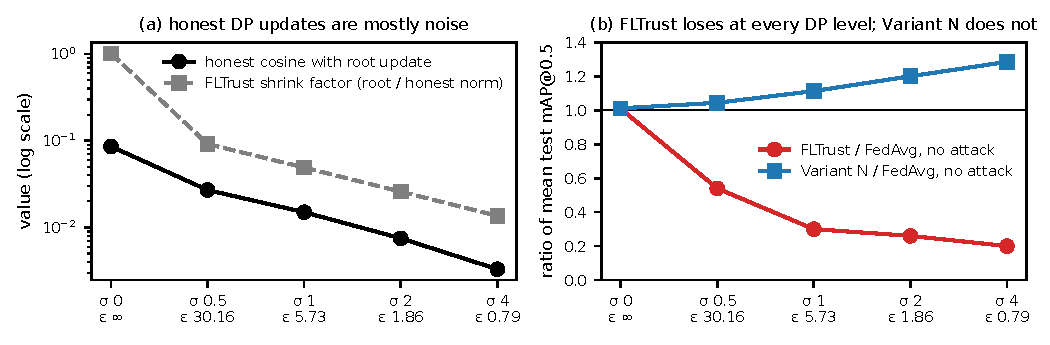
\includegraphics[width=\textwidth]{figs/fig_mechanism.pdf}
\caption{Noise dominance across privacy levels (no attack, 20 seeds, uniform schedule). (a) Mean
cosine between an honest client update and the server's clean root update, and FLTrust's shrink
factor (root-update norm / honest-update norm), log scale. (b) Ratio of mean test \mAP{} to FedAvg
for FLTrust and for Variant N. What to notice: the cosine and the shrink factor both fall by over an
order of magnitude as $\eps$ tightens, and FLTrust's accuracy follows them (Spearman $+1$ over the five
levels). Variant N stays at or above FedAvg in mean.}
\label{fig:mechanism}
\end{figure*}

\subsection{Late-round noise hurts more}
\textbf{Round sensitivity $a_t$ is not flat in any tested configuration and always rises late.} The
noise-pulse test doubles $\sigma$ in a single round $t$ and measures the drop in final validation
\mAP{} against a paired baseline, with 20 seeds per round. It was run on 3 variants (12 or 25
rounds; 65k or 116k trainable parameters) $\times$ 3 noise levels, 3,120 runs in total. 7 of 9 cells
vary significantly (slope and early-vs-late CIs exclude zero). The other 2 are not identifiable,
because the larger model sits near the floor. None is flat. At P the drop rises from $+0.014$
(round 1) to $+0.187$ (round 12) on a baseline of 0.258. The slope is $+0.0100$ per round
[$+0.0088$, $+0.0112$]. The same shape appears on CIFAR-10 and VisDrone (Fig.~\ref{fig:pulse}). At 25
rounds the sensitivity is flat for rounds 1--20 and concentrated in the last $\sim$5. What to notice:
the last round alone accounts for most of the sensitivity on all three datasets.

\begin{figure}[t]
\centering
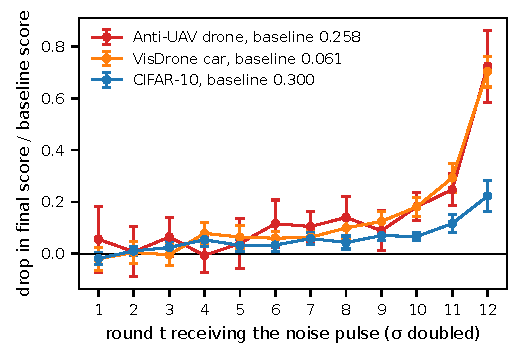
\includegraphics[width=\columnwidth]{figs/fig_pulse.pdf}
\caption{Round sensitivity $a_t$: drop in final validation score when $\sigma$ is doubled in one round,
divided by the baseline score; 20 paired seeds per round, 95\% CI; $\eps = 1.86$, 12 rounds. What
to notice: all three datasets rise late; the drone and VisDrone profiles almost coincide, while
CIFAR-10's rise is about three times weaker relative to its baseline.}
\label{fig:pulse}
\end{figure}

\subsection{Main comparison}
\textbf{At P, the tuned decaying schedule (A2) beats uniform by $+0.0139$ \mAP{} [$+0.0076$,
$+0.0202$] on 16/20 seeds, a relative gain of 23.5\%. The theory schedule (A3) gains $+0.0144$
[$+0.0026$, $+0.0262$], also on 16/20 seeds. Neither learned agent helps
(Table~\ref{tab:methods}).} The feedback agent A5 ties uniform ($-0.0005$ [$-0.0124$, $+0.0115$],
equivalent within $\pm0.02$). It loses to A2 ($-0.0144$, 5/15, Holm $p = 0.011$) and to A3 ($-0.0149$,
4/16, Holm $p = 0.0013$). The blind agent A4 collapses to 0.000 on all 40 test runs at P and S2: it
front-loads spending and is forced to $\sigma = 20$ in late rounds (Fig.~\ref{fig:schedules}).
Under the pre-registered primary family the verdict is that learned allocation does not help. The
A2 and A3 comparisons with uniform were registered as secondary, so they are unadjusted.

\begin{table*}[t]
\centering
\caption{All allocation methods on the Anti-UAV drone task. Mean test \mAP{} over 20 paired seeds.
All methods at an operating point spend the same worst-client $\eps$ (matched to $\pm0.003$).
``Genuine'' means significantly better than uniform \emph{and} than the better of A2/A3 (fixed in
advance: A3 at P, A2 at S1/S2), Holm-adjusted within each phase's family.}
\label{tab:methods}
\begin{tabular}{@{}lllll@{}}
\toprule
Method & P ($\eps$ 1.86) & S1 ($\eps$ 2.72) & S2 ($\eps$ 0.79) & Genuine improvement?\\
\midrule
A1 uniform & 0.0592 & 0.1050 & 0.0143 & reference\\
A2 exponential decay (tuned) & 0.0731 & \textbf{0.1105} & \textbf{0.0254} & beats uniform at P, S2 (16/4); S1 n.s.\ (14/6)\\
A3 theory, $\rho_t\propto\sqrt{a_t}$ & \textbf{0.0736} & 0.0802 & 0.0213 & beats uniform at P, S2 (16/4); \emph{loses} at S1 (3/17)\\
A4 DDPG, blind & 0.0000 & 0.1078 & 0.0000 & no: collapses at P and S2 (0/20)\\
A5 TD3+GRU, feedback & 0.0587 & 0.0981 & 0.0113 & no: loses to A2/A3 at P (5/15, 4/16)\\
A7 Bayesian optimisation & 0.0747 & 0.1060 & 0.0129 & no: beats uniform at P, ties A2/A3; loses to A2 at S2 (1/19)\\
A5-relative ($\pm20\%$ around A3) & 0.0708 & 0.0921 & 0.0208 & no: ties A2/A3 at P, S2; loses to A2 at S1 (3/17)\\
\bottomrule
\end{tabular}
\end{table*}

\begin{figure*}[t]
\centering
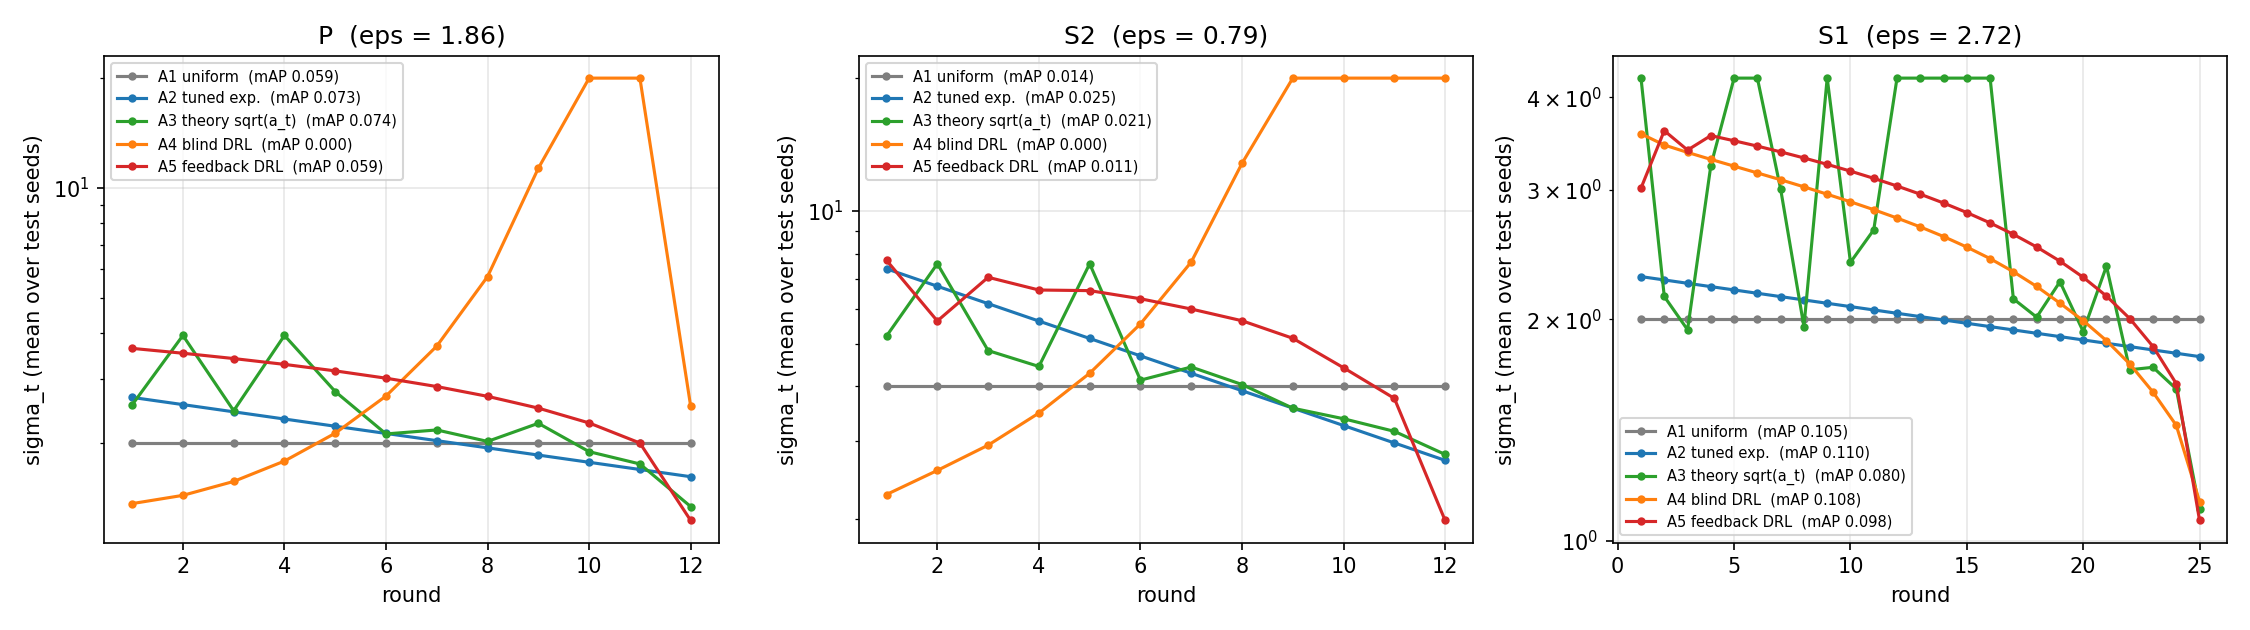
\includegraphics[width=\textwidth]{figs/phase4_schedules.png}
\caption{Deployed noise schedules $\sigma_t$ (mean over the 20 test seeds; log scale) at P, S2 and S1,
with each arm's test \mAP{}. What to notice: A2 and A3 decay gently; A4 front-loads spending and is
forced to $\sigma = 20$ late (0.000 \mAP{}); A5 sits at the most back-loaded schedule its action
range allows (pinned at the minimum action) and does not beat uniform on test; at S1 A3 inherits
noisy $a_t$ estimates (spikes at the cap $\sigma = 4.25$). Regenerate as vector for the final version.}
\label{fig:schedules}
\end{figure*}

\textbf{At the secondary points the picture is weaker.} At S2 ($\eps = 0.79$), A2 and A3 again beat
uniform ($+0.0111$ and $+0.0071$, 16/4 each), near the floor. At S1 (25 rounds) the decay gain is not
significant ($+0.0055$ [$-0.0005$, $+0.0114$]). There the theory schedule loses to uniform ($-0.0248$
[$-0.0371$, $-0.0125$], 3/17). Its per-round $a_t$ estimates are noisy, many are floored, and the
floored rounds receive the capped $\sigma = 4.25$.

\subsection{Generalisation beyond the drone data}
\textbf{The direction replicates on VisDrone, but the size of the gain does not transfer reliably.}
\begin{itemize}
  \item \emph{VisDrone (car, tile-level).} Same client sizes, so $\eps = 1.86$. A2 beats uniform by
  $+0.0037$ [$+0.0020$, $+0.0054$], 17/3, Holm $p = 0.0006$, a $+10.5\%$ relative gain. The
  pre-registered ``drone-like'' line was 10\%, so this classification is narrow (CI of the relative
  gain $+5.6\%$ to $+15\%$). A3 ties uniform, again because its early-round $a_t$ estimates are
  floored. Kiani et al.'s rule (A6) wins ($+0.0032$, 17/3).
  \item \emph{CIFAR-10.} The same $a_t$ shape appears, but the gain is $+0.0050$ accuracy (16/4,
  Holm $p = 0.088$), $+1.7\%$ relative. All primary comparisons are equivalent within $\pm0.02$, and
  A6 is the worst arm (loses to A2 on 19/20 seeds).
  \item \emph{Pascal VOC~\cite{everingham2010voc}.} Stopped at the pre-registered quality gate: the
  frozen-trunk head reaches only 0.058--0.074 \mAP{} without noise under three configurations (bar
  0.104). An oracle check (0.990) ruled out a scoring bug.
\end{itemize}
A non-flat $a_t$ is therefore necessary for a benefit but does not set its size.

\subsection{Nothing for learning to add}
\label{sec:res-learn}
\textbf{Neither server-side signal tested tells a policy anything the schedule does not.}
\begin{itemize}
  \item \emph{Proxy loss.} There is large between-seed spread early (up to 28.6\% of total training
  progress under A3), but it does not persist. Where the spread is large (rounds 1--5), a seed's loss
  barely predicts its final loss ($\rho \approx 0$). Where it persists (rounds 8--11, $\rho$ 0.5--0.75),
  the spread is 4--8\%.
  \item \emph{Gradient norm (3-round rolling mean).} It does not predict final validation \mAP{}
  (best $|\rho| = 0.30$ in rounds 1--8 under A3). It moves in lockstep with the round's own noise dose
  ($r = +0.68$ [0.51, 0.85]).
\end{itemize}
A5's deployed schedule was identical under every attack and aggregator in Section~\ref{sec:res-trust}
(max $\sigma$ difference $2\times10^{-6}$): it ignores its inputs.

Two alternatives with the same compute also fail to beat the fixed schedules.
\begin{itemize}
  \item \emph{Bayesian optimisation (A7).} It beats uniform at P ($+0.0155$ [$+0.0050$, $+0.0261$],
  Holm $p = 0.019$) but ties A3 ($+0.0011$) and A2 ($+0.0016$). Its best simulator scores were mostly
  the maximum of noisy trials: on fresh seeds the S2 pick was already worse than uniform in the
  simulator ($-0.050$).
  \item \emph{A5-relative.} It ties A3 ($-0.0028$, EQUIVALENT) and A2 at P, and loses to A2 at S1
  ($-0.0184$, 3/17). Its training reward never rose at any operating point. Its adjustments are
  structured and do vary with feedback (between-seed sd 0.051 at P), but they do not improve accuracy.
\end{itemize}

\subsection{More rounds at fixed privacy}
\label{sec:res-rounds}
\textbf{At fixed $\eps = 1.86$, more rounds do not close the gap to the no-DP model; past 25 rounds
they widen it (Fig.~\ref{fig:rounds}).} A2 scores 0.0731, 0.0861, 0.0573 and 0.0401 at 12, 25, 50 and
100 rounds; uniform follows the same curve. The no-DP model scores 0.250, 0.321, 0.340 and 0.330, so
the private share of it falls from 0.29 to 0.12. In the pre-registered family:
\begin{itemize}
  \item $25-12$: $+0.0131$, TIE.
  \item $50-25$: $-0.0288$ [$-0.0457$, $-0.0119$], 7/13, LOSS.
  \item $100-50$: $-0.0172$, 6/14, Holm $p = 0.056$, TIE.
\end{itemize}
The verdict is therefore ``noise ceiling / plateau'', not formally ``declining''. A2's advantage over
uniform is constant: $+0.014$, $+0.012$, $+0.012$, $+0.013$, with 15--17 wins out of 20 at every $R$.
Fixing $\eps$ forces the per-round $\sigma$ up as $R$ grows (uniform 2.00 $\to$ 5.15). The final proxy
loss of the DP model rises with $R$ (0.89, 1.11, 1.43), while the no-DP model reaches 0.43--0.45 at
every $R$.

\begin{figure*}[t]
\centering
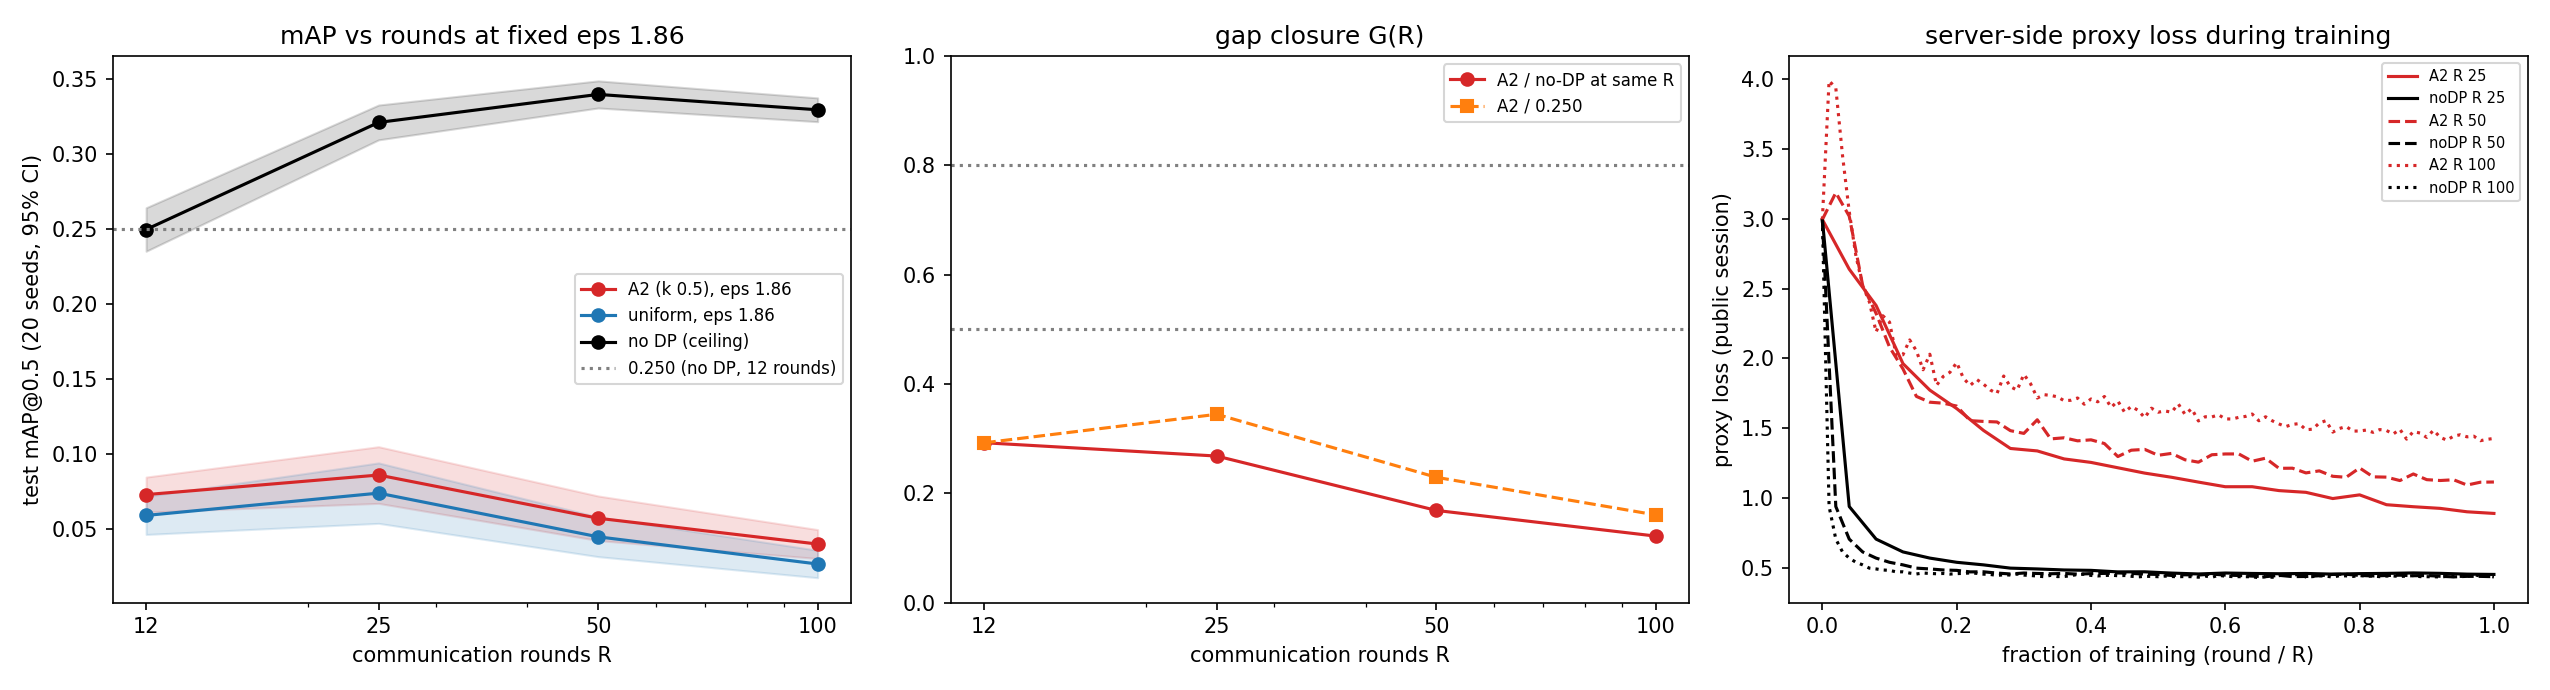
\includegraphics[width=\textwidth]{figs/phase4g_rounds.png}
\caption{Rounds at fixed worst-client $\eps = 1.86$. Left: test \mAP{} (20 seeds, 95\% CI) vs the number
of rounds for A2, uniform, and no DP. Middle: gap closure $G(R)$ = A2 / no-DP at the same $R$.
Right: server-side proxy loss during training. What to notice: the DP curves peak at 25 rounds while
no DP keeps rising to 50, and the DP proxy loss ends higher the longer the run. Regenerate as vector
for the final version.}
\label{fig:rounds}
\end{figure*}

% -----------------------------------------------------------------------------
\section{Results II: Trust-Based Robustness Under DP}
\label{sec:res-trust}

\subsection{FLTrust fails at every privacy level}
\textbf{At $\eps = 1.86$, FLTrust loses to FedAvg with no attack ($-0.0441$ [$-0.0596$, $-0.0286$],
2/18), a 75\% loss of accuracy. It also loses under ALIE (0/20), IPM (1/19) and Fang (3/17).} The
classical rules also cost accuracy without attack: median $-0.0214$ (4/16) and Krum $-0.0507$ (2/18),
both LOSS. Across privacy levels:
\begin{itemize}
  \item FLTrust loses to FedAvg without attack at $\eps$ = 30.16 ($-0.082$, 0/20), 5.73 ($-0.093$,
  0/20) and 0.79 ($-0.011$, 3/17).
  \item It loses under every attack except Fang at $\eps = 0.79$, where it ties at the floor.
  \item Its accuracy relative to FedAvg tracks the honest cosine and the shrink factor exactly
  (Spearman $+1.00$ for each, over five levels; Fig.~\ref{fig:mechanism}).
  \item Without DP it ties FedAvg and beats it under Fang ($+0.045$, 16/4), as designed.
\end{itemize}
What to notice: the failure is specific to DP, and it grows as privacy tightens.

\subsection{A noise-aware repair, and its limits}
\textbf{The two possible culprits can be separated. Correcting the cosine (Variant L) does not help;
correcting the norm target (Variant N) does.} Variant L still loses to FedAvg in all four conditions
($-0.042$, $-0.036$, $-0.058$, $-0.023$). Variant N rescales each update to
$N_t = \sqrt{\|g_0\|^2 + Dv_t}$ instead of $\|g_0\|$ and keeps FLTrust's trust weights. At
$\eps = 1.86$ it ties FedAvg with no attack ($+0.012$ [$-0.008$, $+0.032$], 9/11), under ALIE
($+0.004$) and under IPM ($-0.009$), and beats it under Fang ($+0.026$ [$+0.008$, $+0.045$], 15/5).
It beats plain FLTrust in all four conditions (17/3 to 20/0). The ties are not equivalences: the CIs
reach $+0.032$ and $-0.025$. The no-attack mean gain comes largely from one seed (per-seed range
$-0.026$ to $+0.131$; Fig.~\ref{fig:perseed}).

\textbf{Variant N does not recover at every privacy level.} Pre-registered family F8 gives:
\begin{itemize}
  \item $\sigma = 0$ ($\eps=\infty$): recovers; Variant N is identical to FLTrust there on 80/80 runs.
  \item $\sigma = 0.5$ ($\eps = 30.16$): recovers.
  \item $\sigma = 1$ ($\eps = 5.73$): loses under IPM ($-0.030$ [$-0.052$, $-0.009$], 6/14).
  \item $\sigma = 4$ ($\eps = 0.79$): loses under ALIE ($-0.011$, 1/19, near the floor).
\end{itemize}

\subsection{An adaptive adversary, and why a weight cap does not stop it}
\label{sec:res-adaptive}
\textbf{An attacker who knows Variant N's rule and the root update drives it from 0.071 to 0.0005
\mAP{}.} At three decimals 18 of 20 seeds score 0.000, and 16 are exactly zero. This is a LOSS
against FedAvg under the same attack ($-0.013$ [$-0.023$, $-0.003$], 1/18), and below plain FLTrust
(0.0055). Because Variant N gives every update the same norm, weight is decided by trust alone. Honest
trust scores sum to only $\sim$0.04 per round, so an update with cosine $c \approx 0.3$--$0.5$ takes
about 60--73\% of the weight. The attack is strong in general: it also cuts FedAvg from 0.059 to
0.014.

\textbf{Capping any client's normalised trust weight at $\kappa = m/8$ does not fix this.} We tested
$m = 2$, 1.5 and 1. The cap redistributes excess weight by water-filling and drops it when too few
clients have positive trust. It works exactly as designed: the attackers' share is held at
$2\kappa$ = 50\%, 37.5\% and 25\%, down from 73\%. Yet the model still collapses
(Table~\ref{tab:cap}, Fig.~\ref{fig:cap}).
\begin{itemize}
  \item ``Collapse prevented'' (capped vs uncapped under the attack) ties at every margin.
  \item At $m = 1.5$ the capped system loses to FedAvg (0/19).
  \item A cap-aware attacker, who picks the smallest cosine that still reaches the cap, is no stronger.
  \item The cap costs nothing in the standard conditions (no LOSS), and at $m = 1$ it even improves
  robustness to ALIE ($+0.031$ [$+0.012$, $+0.050$], 15/5).
\end{itemize}
The post-hoc reading of Proposition~\ref{prop:noise} explains this. Once honest updates are mostly
noise, a coherent update needs only $\sim$2.5\% of the weight to dominate the aggregate's useful
direction. FedAvg, which gives the attackers 17.1\%, is itself badly hurt.

\begin{table*}[t]
\centering
\caption{Per-client trust-weight cap on Variant N at $\eps = 1.86$. Mean test \mAP{}, 20 paired
seeds; [seeds at 0.000]. Bottom rows: Holm-adjusted tests within each margin (pre-registered family,
6 tests).}
\label{tab:cap}
\begin{tabular}{@{}lccccc@{}}
\toprule
& Variant N, no cap & cap $2/8$ & cap $1.5/8$ & cap $1/8$ & FedAvg\\
\midrule
No attack & 0.071 & 0.072 & 0.071 & 0.065 & 0.059\\
ALIE & 0.044 & 0.051 & 0.066 & \textbf{0.074} & 0.039\\
IPM & 0.070 & 0.068 & 0.079 & 0.081 & 0.078\\
Fang & 0.070 & 0.067 & 0.073 & 0.074 & 0.044\\
Trust-capture & 0.0005 [18] & 0.0004 [19] & 0.0000 [20] & 0.0058 [14] & 0.0137 [7]\\
Trust-capture, cap-aware & -- & 0.0003 [18] & 0.0014 [12] & -- & --\\
Attackers' weight share & 73\% & 50\% & 37.5\% & 25\% & 17.1\% (data)\\
Capped vs no cap, trust-capture & -- & tie & tie & tie & --\\
vs FedAvg, trust-capture & $-0.013$, 1/18, LOSS & $-0.013$, tie & $-0.014$, 0/19, LOSS & $-0.008$, tie & --\\
\textbf{Genuine fix?} & -- & \textbf{no} & \textbf{no} & \textbf{no} & --\\
\bottomrule
\end{tabular}
\end{table*}

\begin{figure*}[t]
\centering
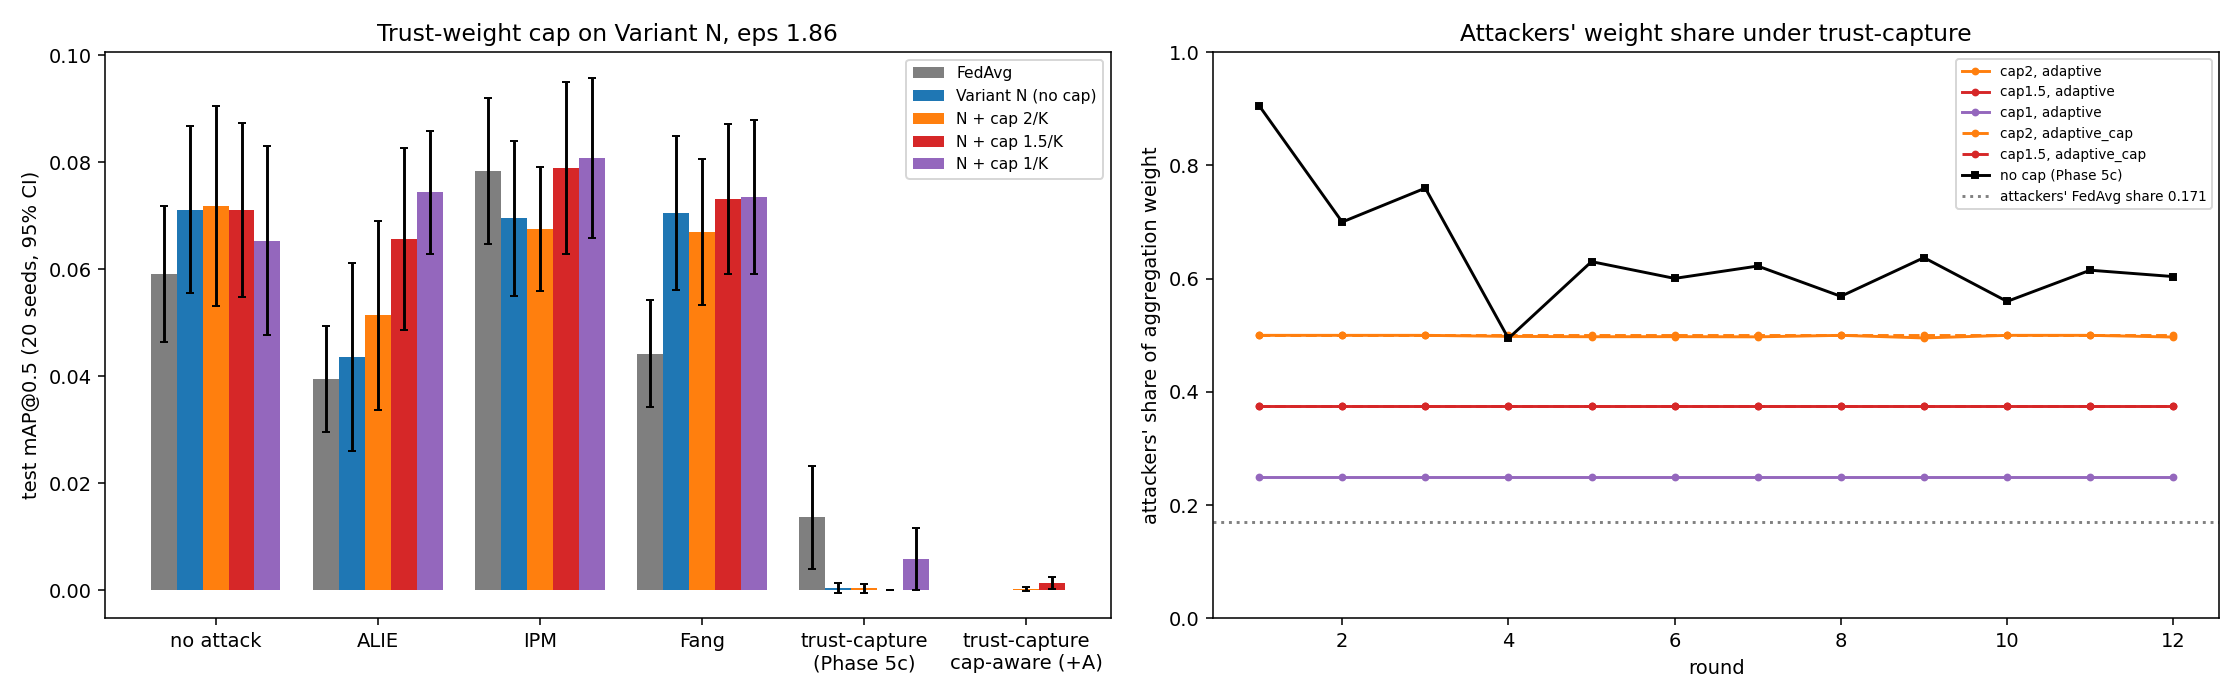
\includegraphics[width=\textwidth]{figs/phase5d_trust_cap.png}
\caption{Left: mean test \mAP{} (20 seeds, 95\% CI) of FedAvg, Variant N and three trust caps under no
attack, the three standard attacks, the trust-capture attack and its cap-aware variant. Right: the
attackers' share of aggregation weight per round under trust-capture. What to notice: the caps hold
the attackers' share flat at exactly $2\kappa$, yet every capped bar under trust-capture is at the
floor. Regenerate as vector for the final version.}
\label{fig:cap}
\end{figure*}

\begin{figure*}[t]
\centering
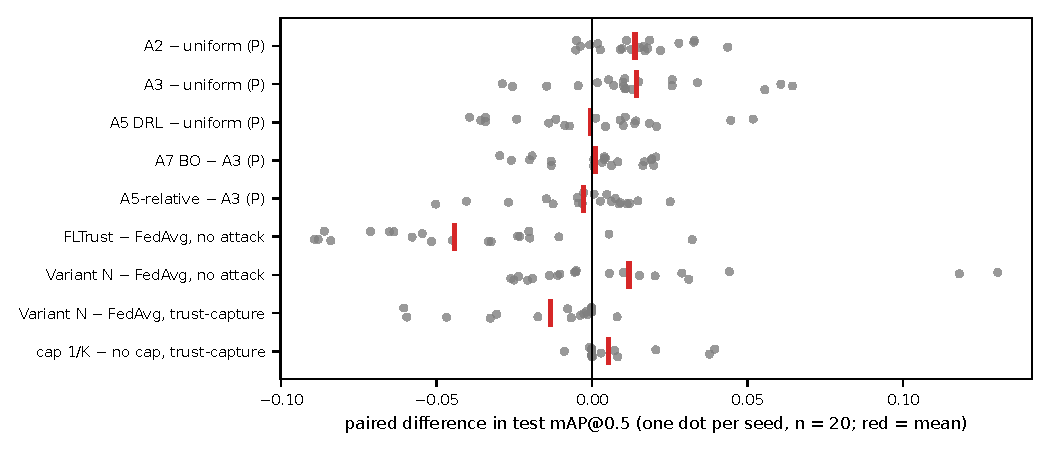
\includegraphics[width=\textwidth]{figs/fig_perseed.pdf}
\caption{Per-seed paired differences in test \mAP{} for the headline comparisons ($n = 20$ each, one dot
per seed, red bar = mean; P unless stated). What to notice: the decay schedules' gain over uniform
is consistent (16/20 seeds), the learned and searched schedules scatter around the fixed ones, and
Variant N's mean gain without attack rests partly on one seed ($+0.131$).}
\label{fig:perseed}
\end{figure*}

% -----------------------------------------------------------------------------
\section{Failed Predictions, Null Results and Retractions}
\label{sec:res-failed}

\textbf{Retraction: the FL$\times$DP interaction.} An early 2$\times$2 experiment found that DP hurts
far more inside FL than centrally (interaction $-0.120$ [$-0.178$, $-0.062$], 0/10). That run used a
clipping bound $C = 45.8$ measured on the untrained model. After round 1 this bound clipped only
0.3--0.5\% of samples, while the noise stayed sized for it. With the calibrated $C^\ast$ the
interaction reverses sign: $+0.135$, $+0.330$ and $+0.201$ at $\sigma$ = 1, 2, 4, 10/10 seeds each.
Under calibrated clipping, central DP-SGD suffers more than federated DP at equal $\sigma$; the
federated clients have larger $\eps$ at the same $\sigma$, so the cells are matched on $\sigma$,
not on $\eps$. Every result in this paper uses $C^\ast$.

\textbf{Failed pre-registered predictions} (Table~\ref{tab:scorecard}).

\begin{table}[t]
\centering
\caption{Pre-registered predictions that failed. Held predictions are listed in the per-phase
reports in the repository.}
\label{tab:scorecard}
\begin{tabular}{@{}p{0.47\columnwidth}p{0.43\columnwidth}@{}}
\toprule
Prediction & Outcome\\
\midrule
Rounds: flat accuracy at fixed $\eps$ (H3) & held as ``no gain'', but accuracy \emph{fell} past 25 rounds\\
A5-relative beats A5 at P & $+0.012$, Holm $p = 0.14$: tie\\
A5-relative ignores feedback (sd $<0.02$) & sd 0.051--0.085: it reacts\\
Variant N only partly recovers at $\eps = 1.86$ & failed in the good direction: full recovery\\
Variant N recovers at every $\eps$ & fails at $\sigma=1$ (IPM) and $\sigma=4$ (ALIE)\\
Trust-capture takes $\ge 85\%$ of weight & $\sim$60--73\%\\
Trust-capture hurts FedAvg much less & FedAvg 0.059 $\to$ 0.014\\
Weight cap prevents collapse (H5) & no margin does\\
Cap at $m=2$ loses to FedAvg & tie (Holm $p = 0.064$)\\
Cap at $m=1.5$ is a narrow fix & fails; LOSS vs FedAvg\\
\bottomrule
\end{tabular}
\end{table}

\textbf{Null results} reported as such:
\begin{itemize}
  \item learned allocation (A4, A5) vs uniform;
  \item BO and A5-relative vs the fixed schedules;
  \item CIFAR-10 replication (equivalent);
  \item FedProx~\cite{li2020fedprox} ($\mu$ 0.01--0.3 tie at $\sigma = 1, 2$; $\mu = 1$ loses at $\sigma = 2$, $-0.050$, 1/10);
  \item the schedule's effect on attack damage under FLTrust (6/6 equivalent within $\pm0.008$).
\end{itemize}

\textbf{Discarded implementations} (all fixed by dated amendments before the reported runs):
\begin{itemize}
  \item the agent action mapping first measured spend in a zCDP-style unit that understated the true
  cost under subsampling;
  \item the TD3+GRU critic target dropped the first observation;
  \item the first simulator could not train;
  \item an unclipped FLTrust root update diverged;
  \item a first A5-relative training run stalled on memory and was restarted from scratch with the
  same seeds.
\end{itemize}

\textbf{Unexpected effect.} IPM \emph{helps} FedAvg under DP ($+0.019$, 16/4 seeds better). Its two
updates are $-0.5\times$ the mean of six noisy updates, so they carry about $\sqrt{6}$ less noise.
Replacing two noisy updates with them reduces the aggregate noise more than the reversed direction
hurts. Without DP, IPM has no effect.

\textbf{Closest prior method on its own benchmark.} \missing{a reproduction of Kiani et
al.~\cite{kiani2025timeadaptive} on MNIST/FMNIST/Adult at client-level DP. We implemented their rule
only inside our setting (A6), via $\sigma$ instead of client subsampling.}

% -----------------------------------------------------------------------------
\section{Discussion}
\label{sec:discussion}

\textbf{One fact, two consequences.} At $\eps \le 3$ with $D = 65{,}221$, each honest update is noise
plus a faint signal (cosine 0.0075). For allocation, the accuracy cost of noise is set by where it
lands: late noise reaches the final model with little time to average out (Fig.~\ref{fig:pulse}). A
fixed decaying schedule captures this. A feedback policy would need a signal that reveals more than
the schedule already implies. The two server-side signals we tested do not: one is transient, the
other tracks the noise just injected. For robustness, a defence that reads per-update geometry has
almost nothing honest to read. FLTrust's norm equalisation then throws away 97\% of every update.
Once the norm is repaired, any coherent update dominates at a weight far below what per-client caps
can enforce. The two halves meet at Proposition~\ref{prop:noise}.

\textbf{Practical recommendations.}
\begin{enumerate}
  \item Use a fixed, gently decaying noise schedule ($k$ between 0.25 and 1, tuned on validation data) rather than uniform when privacy is
  strong and accuracy is off the floor: $+23.5\%$ on the drone task and $+10.5\%$ on VisDrone, at no
  privacy or training cost (Table~\ref{tab:methods}).
  \item Do not train a reinforcement-learning or search-based allocator for this regime. It cost 1--8
  GPU-hours per agent and gave no gain, and the blind DDPG agent collapsed (Table~\ref{tab:methods}).
  \item Do not raise the round count to buy accuracy at a fixed $\eps$. Beyond about 25 rounds it
  lowered accuracy (Fig.~\ref{fig:rounds}).
  \item Do not deploy FLTrust unmodified under DP. Plain FedAvg was the best of FedAvg, FLTrust,
  median and Krum under every attack at $\eps = 1.86$ (Section~\ref{sec:res-trust}).
  \item If a trust-based rule is used, rescale to the known DP norm (Variant N). Treat it as a utility
  fix only: it is broken by an attacker who knows the rule (Section~\ref{sec:res-adaptive}).
  \item Per-client weight caps are cheap and help against ALIE, but they are not a defence against a
  coherent adaptive attacker (Table~\ref{tab:cap}).
\end{enumerate}

\textbf{Relation to prior work.} Our allocation direction agrees with Kiani et
al.~\cite{kiani2025timeadaptive}. Their rule is the worst arm on CIFAR-10 in our setting and wins on
VisDrone, so its value is dataset-dependent at strong privacy. Our robustness results are consistent
with Guerraoui et al.'s dimension argument~\cite{guerraoui2021dpbyz}. They do not contradict
FLTrust~\cite{cao2021fltrust} in its noise-free regime.

\textbf{Tension.} The repair that restores utility (equal norms) is what lets the adaptive attacker
win. The original FLTrust's shrinkage was also a crude defence: plain FLTrust lost less to the
trust-capture attack (0.0055) than Variant N did (0.0005). Under DP, utility and robustness pull the
norm target in opposite directions.

% -----------------------------------------------------------------------------
\section{Limitations}
\label{sec:limits}
\begin{itemize}
  \item \textbf{Privacy unit.} Every $\eps$ is frame-level. Consecutive frames of a recording are
  highly correlated, so a recording-level guarantee is much weaker (group privacy).
  \item \textbf{Unaccounted tuning.} A2's $k$ was tuned on the validation pool, and A3's $a_t$ came
  from 3,120 training runs on client data. Their privacy cost~\cite{papernot2022hyperparam} is not in
  the reported $\eps$.
  \item \textbf{One primary dataset.} All security results and the main allocation results use
  Anti-UAV. Allocation replicates on VisDrone (narrowly) and only in direction on CIFAR-10. VOC
  could not be tested.
  \item \textbf{Low absolute accuracy and a validation-to-test shift.} Uniform scores 0.059 on test
  vs $\sim$0.29 on validation. The test sessions hold many tiny targets (median box 110 vs 621
  px$^2$). Paired differences are unaffected, but absolute gains are small (+0.014 \mAP).
  \item \textbf{Small trainable model} (65,221 parameters, frozen trunk). Effects may depend on $D$.
  \item \textbf{Test-pool reuse.} The same 12 test sessions serve all phases. Holm corrects within
  pre-registered families, not across phases.
  \item \textbf{Threat model.} Two fixed attackers (17.1\% of the data). The root set covers 2 of 4
  environments. The adaptive attacker is omniscient (it knows $g_0$); attackers who must estimate
  $g_0$ are untested. No DP-native robust aggregators were compared.
  \item \textbf{Simulator.} Agents trained in a public-data simulator. Its pseudo-clients reuse
  near-duplicate consecutive frames.
  \item \textbf{Stand-ins.} Kiani et al.'s rule was realised through $\sigma$, not client subsampling.
  VisDrone mAP is tile-level for one class.
\end{itemize}

% -----------------------------------------------------------------------------
\section{Open Problem}
\label{sec:open}
\textbf{How can a server bound a coherent attacker's influence when honest updates are mostly noise?}
Weight-based defences cannot. By Proposition~\ref{prop:noise} the attacker needs only a few percent
of the weight, below any per-client cap that still averages honest noise. Direction-based defences
need the honest direction, which DP hides at the level of a single update. That is the purpose of DP.
A defence would have to accumulate evidence across rounds (an attacker's push is consistent, honest
noise is not), or obtain a server-side signal strong enough to stand in for the honest direction.
Both conflict with what the privacy guarantee removes. We therefore expect the problem to be
structural at strong privacy rather than a matter of tuning.

% -----------------------------------------------------------------------------
\section{Conclusion}
\label{sec:conclusion}
We measured both privacy-budget allocation and trust-based robust aggregation on one differentially
private federated drone detector at worst-client $\eps$ 0.79--2.72. The measurements used
pre-registered rules, 20 paired seeds and Holm correction.
\begin{itemize}
  \item A fixed decaying schedule gave $+0.0139$ \mAP{} ($+23.5\%$) over uniform at $\eps = 1.86$.
  Learned, searched and constrained-learned schedules gave nothing more.
  \item More rounds at a fixed $\eps$ lowered accuracy past 25.
  \item FLTrust lost 75\% of its accuracy to DP noise. Its noise-aware repair was driven to 0.0005
  \mAP{} by a rule-aware attacker, and a 1/8 weight cap still left 0.0058.
\end{itemize}
At strong privacy an honest DP update is almost entirely noise; consequently, all the allocation
gain we could measure comes from placing less noise in later rounds, which a fixed schedule already
captures, while trust-based robust aggregation either drowns the honest signal or hands control to a
coherent attacker.
\emph{Practical advice:} decay the noise with a fixed schedule, and keep FedAvg unless a defence has
been tested against an attacker who knows it.
\emph{Scientific claim:} at strong privacy, what can be learned or defended in federated training is
bounded by how little signal a single noisy update carries.

% -----------------------------------------------------------------------------
\section*{Data and Code Availability}
Pre-registrations, code, per-run result files and analyses are in the \texttt{restart/} directory of
the project repository (branch \texttt{restart}). \missing{public repository URL and dataset licence
statement.}

\bibliographystyle{IEEEtran}
\bibliography{references}

\end{document}
